\let\negmedspace\undefined
\let\negthickspace\undefined
\documentclass[journal]{article}
\usepackage[a5paper, margin=10mm, onecolumn]{geometry}
\usepackage{lmodern} % Ensure lmodern is loaded for pdflatex

\setlength{\headheight}{1cm} % Set the height of the header box
\setlength{\headsep}{0mm}     % Set the distance between the header box and the top of the text

\usepackage{gvv-book}
\usepackage{gvv}
\usepackage{cite}
\usepackage{textcomp}
\usepackage{amsmath,amssymb,amsfonts,amsthm}
\usepackage{algorithmic}
\usepackage{graphicx}
\graphicspath{{./figs/}}
\usepackage{textcomp}
\usepackage{xcolor}
\usepackage{txfonts}
\usepackage{listings}
\usepackage{enumitem}
\usepackage{mathtools}
\usepackage{gensymb}
\usepackage{comment}
\usepackage[breaklinks=true]{hyperref}
\usepackage{tkz-euclide} 
\usepackage{listings}
\usepackage{gvv}                                        
\def\inputGnumericTable{}                                 
\usepackage[latin1]{inputenc}                                
\usepackage{color}                                            
\usepackage{array}                                            
\usepackage{longtable}                                       
\usepackage{calc}                                             
\usepackage{multirow}                                         
\usepackage{hhline}                                           
\usepackage{ifthen}                                           
\usepackage{lscape}
\usepackage{circuitikz}
\tikzstyle{block} = [rectangle, draw, fill=blue!20, 
text width=4em, text centered, rounded corners, minimum height=3em]
\tikzstyle{sum} = [draw, fill=blue!10, circle, minimum size=1cm, node distance=1.5cm]
\tikzstyle{input} = [coordinate]
\tikzstyle{output} = [coordinate]


\begin{document}
	
	\bibliographystyle{IEEEtran}
	\vspace{3cm}
	
\title{5.2.49}
\author{EE25BTECH11047 - RAVULA SHASHANK REDDY}
\maketitle
\hrulefill
\bigskip 

\renewcommand{\thetable}{\theenumi}
\setlength{\intextsep}{10pt}

\textbf{Question:} \\

Solve the system of equations using matrices:
\begin{align*}
3x - y - 2z &= 2, \\
2y - z &= -1, \\
3x - 5y &= 3.
\end{align*}

\textbf{Solution:}\\

Given:
\begin{align}
\myvec{3\\-1\\-2}^{T}\vec{x}&=2,\\
\myvec{0\\2\\-1}^{T}\vec{x}&=-1,\\
\myvec{3\\-5\\0}^{T}\vec{x}&=3\\
\myvec{3 & -1 & -2  \\
0 & 2 & -1  \\
3 & -5 & 0 } \vec{x} &= \myvec{2 \\ -1 \\ 3}\\
R_3\rightarrow R_3-R_1 &\Rightarrow
\myvec{3 & -1 & -2 & 2 \\
0 & 2 & -1 & -1 \\
0 & -4 & 2 & 1}
\end{align}
\begin{align}
R_2\rightarrow \tfrac{1}{2}R_2 &\Rightarrow
\myvec{3 & -1 & -2 & 2 \\
0 & 1 & -\tfrac{1}{2} & -\tfrac{1}{2} \\
0 & -4 & 2 & 1}
\end{align}
\begin{align}
R_1\rightarrow R_1+R_2,\quad R_3\rightarrow R_3+4R_2 &\Rightarrow
\myvec{3 & 0 & -\tfrac{5}{2} & \tfrac{3}{2} \\
0 & 1 & -\tfrac{1}{2} & -\tfrac{1}{2} \\
0 & 0 & 0 & -1}
\\[6pt]
&\implies 0=-1
\end{align}

\[
\text{System inconsistent}\quad\Rightarrow\quad\boxed{\text{No solution}}
\]
\newpage
\begin{figure}
    \centering
    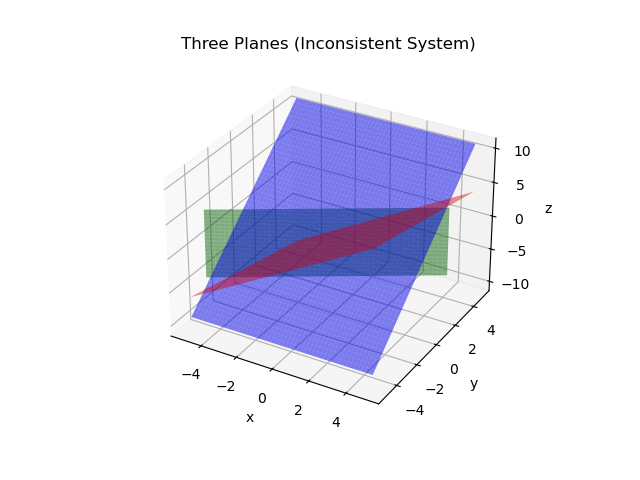
\includegraphics[width=1.0\linewidth]{figs/fig1.png}
    \caption{}
    \label{fig:placeholder}
\end{figure}
\end{document}


